\chapter{Protocol Design}
\label{ch:design}

\section{Design Goals}
\label{sec:design-goals}

Central to the vision of Saturn is the pursuit of zero-configuration consumer access. By ensuring that network connectivity alone grants access to AI services, Saturn removes the traditional barriers of URLs, API keys, and account management. Every protocol decision detailed in this chapter is evaluated against its ability to preserve this property, specifically targeting the elimination of the platform lock-in and per-user key management documented by Syed et al.~\cite{syed2025aiaas}.

\begin{figure}[ht]
\centering
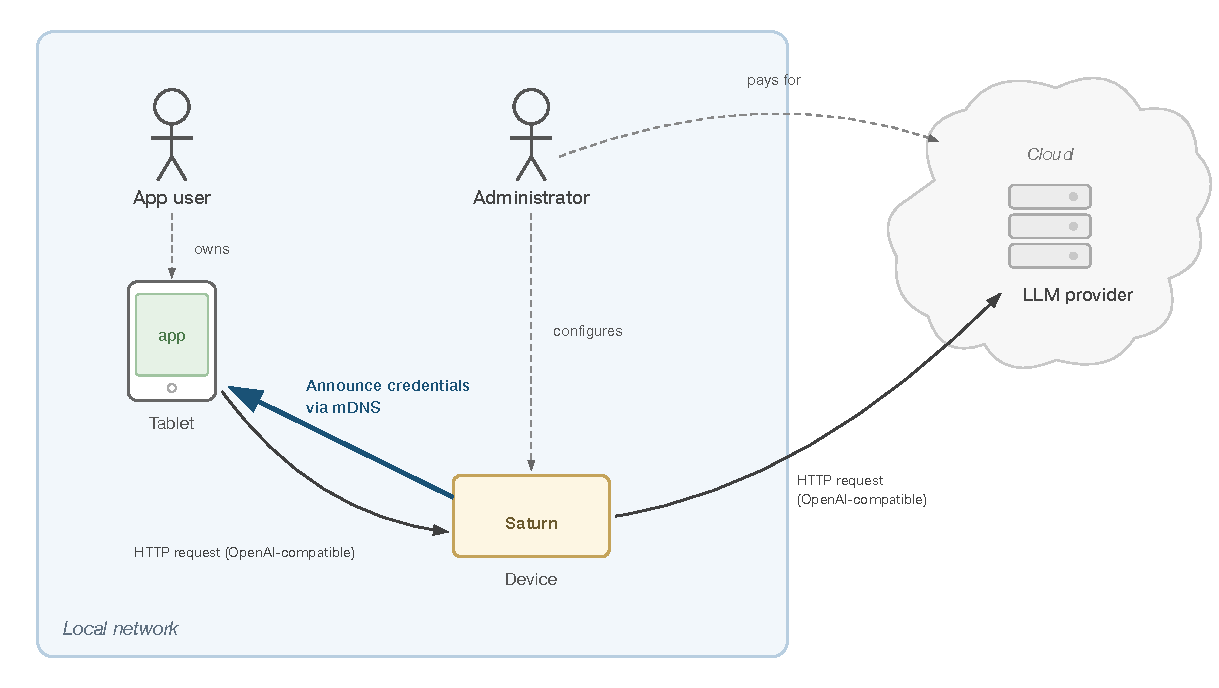
\includegraphics[width=0.85\textwidth]{figures/saturn-network.pdf}
\caption[Overview of Saturn's network architecture.]{Overview of Saturn's network architecture. The Saturn device announces service credentials via mDNS on the local network. Applications discover the service and issue OpenAI-compatible HTTP requests. The administrator configures the device and manages the cloud provider relationship; the app user interacts only with the application.}
\label{fig:saturn-network}
\end{figure}

Saturn must also remain resilient to the volatile landscape of AI inference. To prevent the protocol from locking into a specific backend and ensuring long-term relevance, backend agnosticism is treated as a core requirement. This abstraction allows Saturn to express diverse environments—ranging from local Ollama instances to cloud proxies like OpenRouter through a unified interface. Finally, this high degree of accessibility is balanced against a documented security posture. Rather than ignoring the risks of local credential broadcasting, Saturn’s design explicitly accounts for these trade-offs. As detailed in Section~\ref{sec:security}, the architecture establishes rigorous threat models and mitigations tailored for the trust profiles of homes, offices, and research laboratories.

\section{Audiences}
\label{sec:audiences}

Saturn defines three roles. Three is the minimum decomposition that separates credential management (administrator), integration logic (developer), and usage (end user) into distinct responsibility boundaries. Every design decision identifies which role bears complexity and which roles benefit. Figure~\ref{fig:audiences} summarises each role.

\begin{center}
\fbox{\begin{minipage}{0.9\textwidth}
\begin{singlespace}
\small
\smallskip
\textbf{Administrator.}\quad Deploys and configures Saturn services: selects backends, sets priorities, manages API credentials, and monitors health. The only role that touches configuration files or credentials. In a university department, this is IT staff; in a home, the technically inclined household member. Running Saturn adds one configuration file and one background process---a fixed cost amortized across every other user on the network.

\medskip
\textbf{Application developer.}\quad Integrates Saturn discovery into software. Rather than hard-coding endpoints and requiring users to supply credentials, the developer calls a function like \texttt{discover()} that returns available services with URLs and credentials already populated. No authentication logic, no configuration UI, no billing integration. Chapter~\ref{ch:implementation} details the integration patterns.

\medskip
\textbf{End user.}\quad Interacts with AI-powered applications without awareness that Saturn exists. A student opens a chat application on the campus network, types a question, and receives a response---no API key prompt, no account creation, no settings page. This role performs zero configuration steps.
\smallskip
\end{singlespace}
\end{minipage}}
\captionof{figure}{Saturn's three audience roles and their responsibilities.}
\label{fig:audiences}
\end{center}
\section{Standardizing Endpoint Communication}
\label{sec:standardized-interface}

To ensure seamless interoperability across a landscape of different AI providers, Saturn mandates that every discovered backend adhere to a unified communication protocol. Rather than introducing a proprietary schema, Saturn adopts the OpenAI-compatible REST API as its foundational interface. This grants Saturn immediate compatibility with established backends such as Ollama~\cite{ollama} and OpenRouter~\cite{openrouter}.

To qualify as a valid Saturn \emph{endpoint}, a service must implement a foundational subset of the OpenAI specification, specifically exposing the following three paths:
\begin{itemize}
    \item \texttt{GET /health}: A diagnostic route returning a JSON object to verify service liveness and operational readiness.
    \item \texttt{GET /v1/models}: An enumeration endpoint that provides a list of available models and their metadata in the standardized list-models format.
    \item \texttt{POST /v1/chat/completions}: The primary data exchange route, supporting the full breadth of chat completion requests, including both atomic and multiplexed streaming responses.
\end{itemize}

The adoption of this standard facilitates a "zero-configuration" deployment model: any application designed for OpenAI’s infrastructure can function as a Saturn client, and any compatible backend becomes instantly discoverable. While this introduces a structural dependency on a third-party specification, the stability of the \texttt{/v1/chat/\allowbreak{}completions} interface and its widespread adoption as a \textit{de facto} industry standard mitigate the risks of breaking changes. By prioritizing ubiquitous compatibility over custom extensibility, Saturn minimizes the technical friction typically associated with decentralized service integration.

\section{Service Advertisement}
\label{sec:service-advertisement}
\label{sec:service-type}
\label{sec:txt-schema}

Saturn registers services under the DNS-SD service type \texttt{\_saturn.\_tcp.local.}. The underscore prefix follows DNS-SD naming conventions (RFC~6763~\cite{rfc6763}), the \texttt{\_tcp} transport selector indicates the endpoint communicates over TCP (HTTP), and the \texttt{.local.} domain restricts discovery to the link-local mDNS scope.

Each Saturn service produces the standard DNS-SD record triple (PTR, SRV, TXT) described in Chapter~\ref{ch:background}. Saturn's contribution is the TXT record schema: key-value pairs encoded per RFC~6763 (each pair as a single DNS TXT string, formatted as \texttt{key=value}). Table~\ref{tab:txt-fields} specifies the fields.

\begin{table}[ht]
\centering
\caption{Saturn TXT record fields. Fields marked required must appear in every advertisement.}
\label{tab:txt-fields}
\begin{tabular}{@{}llp{2.8in}@{}}
\toprule
\textbf{Field} & \textbf{Required} & \textbf{Description} \\
\midrule
\texttt{version}           & Yes & Protocol version (currently \texttt{1}) \\
\texttt{api\_type}         & Yes & Backend API format (e.g., \texttt{openai}) \\
\texttt{deployment}        & Yes & One of \texttt{local}, \texttt{cloud}, or \texttt{network} \\
\texttt{priority}          & Yes & Numeric routing preference; lower is preferred \\
\texttt{api\_base}         & Conditional & Base URL of the endpoint. Required when \texttt{deployment=cloud}; for local and network deployments, clients construct the URL from the SRV record's host and port \\
\texttt{ephemeral\_key}    & No  & Current API credential; present only for cloud deployments \\
\texttt{rotation\_interval}& No  & Key rotation period in seconds (default: 300) \\
\texttt{features}          & No  & Comma-separated capability list (e.g., \texttt{chat,vision,tools}) \\
\toprule
\end{tabular}
\end{table}

\label{sec:priorities}
The \texttt{priority} field gives administrators a way to express routing policy without requiring clients to understand that policy. Each beacon advertises a numeric priority, lower numbers indicating higher preference. Clients sort by priority and select the lowest-numbered available service. Consider a lab with a local GPU server and a cloud fallback: the administrator sets the Ollama beacon to priority~1 and the OpenRouter beacon to priority~10. Clients prefer local inference automatically. If the local server goes down, they fall back to the cloud service with no user intervention. The semantics mirror DNS SRV record priority (RFC~6763~\cite{rfc6763}), a convention already familiar to network administrators.

\label{sec:ephemeral-keys}
The \texttt{ephemeral\_key} field addresses a harder problem. Meli et al.~\cite{meli2019secrets} found over 100,000 GitHub repositories containing leaked secrets, 81\% never removed after notification. Static keys fail because every mitigation---detection, rotation, revocation---acts after the damage. Saturn sidesteps this failure class with \emph{ephemeral keys}: time-limited API credentials that a cloud beacon generates, broadcasts in its TXT record, and deletes after expiration. The default lifecycle uses a ten-minute key lifetime and a five-minute rotation interval, creating an overlap window where both current and next key are valid. A key that expires in ten minutes is worthless by the time someone extracts it from a packet capture, commits it to a repository, or pastes it in a chat log. The trade-off is operational: ephemeral keys require the beacon to maintain an active session with the cloud provider's key provisioning API. If the beacon loses connectivity, it cannot rotate keys, and the current key eventually expires without replacement. Section~\ref{sec:security} analyzes this and other failure modes.

DNS-SD imposes a 255-byte limit per TXT string (RFC~6763~\cite{rfc6763}). After the \texttt{ephemeral\_key=} prefix, approximately 240 characters remain for the credential itself. JWT tokens from OpenRouter and DeepInfra fit; full X.509 certificates do not. I chose to carry credentials inline in the TXT record rather than requiring clients to fetch them from an HTTPS bootstrap endpoint, because a bootstrap endpoint would reintroduce the infrastructure dependency Saturn exists to eliminate. The constraint is that credential formats must be compact enough for a single TXT string.

\label{sec:discovery-flow}
With the advertisement defined, the discovery flow replaces the configuration file or environment variable that would otherwise contain an API URL and key. Four steps execute without user interaction:

\begin{enumerate}
    \item \textbf{Browse}: The client queries for PTR records of type \texttt{\_saturn.\_tcp.local.}. All beacons on the local network respond with their instance names.
    \item \textbf{Resolve}: For each instance, the client retrieves the SRV record (hostname, port) and TXT record (metadata).
    \item \textbf{Select}: The client sorts by \texttt{priority} (ascending), optionally filters by \texttt{features} or \texttt{deployment} type, and selects the preferred service.
    \item \textbf{Connect}: For cloud deployments, the client uses \texttt{api\_base} and attaches the \texttt{ephemeral\_key} as a Bearer token. For local and network deployments, it constructs the URL from the SRV record (e.g., \texttt{http://\{host\}:\{port\}/v1}).
\end{enumerate}

\section{Beacons}
\label{sec:beacon-architecture}

In the absence of a centralized registry, Saturn facilitates endpoint discovery through a decentralized \emph{beacon} mechanism. Leveraging the Multicast DNS (mDNS) protocol, a beacon broadcasts critical service metadata—including endpoint URLs, API specifications, priority metrics, and authentication requirements—without intercepting or proxying the underlying API traffic. By strictly bifurcating the discovery layer from the data plane, this architecture ensures that clients establish direct peer-to-peer connections with the advertised services.

Beacons are categorized by their deployment scope. A \emph{local} beacon facilitates service discovery within a shared network namespace or LAN, such as a local LLM instance. Conversely, a \emph{cloud} beacon serves as a bridge to remote environments (e.g., OpenRouter), distributing ephemeral credentials that allow network participants to use administrative accounts without individual credential management. While a proxy-based approach would offer native rate limiting and centralized logging, such features demand hardware resources and observational access that contradict Saturn's core objectives. By delegating usage auditing to external reverse proxies at the endpoint level, Saturn maintains a lean, non-intrusive discovery fabric that eliminates the beacon as a single point of failure or a surveillance chokepoint.

\section{Security}
\label{sec:security}

Saturn deliberately trades enterprise-grade verification for zero-configuration access. Two threat models define the boundaries of that trade-off. The mitigations described here are design-time claims; Chapter~\ref{ch:evaluation} evaluates whether they hold in practice.

\subsection{Threat Model 1: Corporate Data Collection}
\label{sec:threat-corporate}

I do not want companies like OpenAI or Anthropic collecting my prompts, conversation histories, or usage patterns. This is the first threat Saturn addresses: a user's AI interactions flow to a cloud provider who retains, analyzes, or monetizes them.

Saturn addresses this threat concretely: an administrator deploys a local inference server---Ollama with an open-weights model---and sets its priority higher than any cloud beacon. Users on the network route to the local service automatically. Their prompts never leave the LAN. This works because the protocol is backend-agnostic; it does not prescribe what runs behind the endpoint.

The limitation is capacity. Local inference requires hardware that matches or approximates the capability of cloud models. A university department can justify a GPU server; a household typically cannot. When the local model is insufficient and the user falls back to a cloud endpoint, Saturn provides no additional data protection beyond what the cloud provider offers. Saturn enables the administrator to make local inference the default path, but it cannot guarantee that path is always available.

\subsection{Threat Model 2: Untrusted Administrator}
\label{sec:threat-admin}

I do not trust the system administrator of my office or house not to snoop. The sysadmin controls the beacon and could route traffic through a logging proxy, advertise a malicious endpoint, or retain copies of ephemeral keys.

The administrator is, by design, the trusted party, so Saturn provides limited mitigation here. The administrator who runs only a beacon cannot see prompts or responses, because API traffic flows directly from client to endpoint. The administrator sees only the metadata broadcast in TXT records---metadata the administrator created in the first place.

An administrator who controls both the beacon and the endpoint, however, has full access to all traffic. Saturn cannot protect against this scenario without introducing user-level authentication, which would destroy the zero-configuration property. This is the fundamental trade-off the architecture makes: Saturn trusts the network in the same way that connecting to office WiFi trusts the network operator with DNS resolution and IP routing. Ward and Beyer~\cite{ward2014beyondcorp} argued in BeyondCorp that networks should never be trusted; Saturn disagrees for its target environment of homes, offices, and campus labs where the network operator is a known party and the alternative---per-user credential management---creates the access barriers Saturn exists to remove.

\subsection{Broadcast Exposure}
\label{sec:broadcast-exposure}

Any device on the local network can observe Saturn's mDNS announcements---the broadcast exposure that Section~\ref{sec:mdns-dnssd} documented applies here. For local deployments, the exposed information is limited to service existence and location. For cloud deployments, the TXT record also contains an ephemeral API key readable by any network participant.

Two mechanisms bound the financial exposure: the ephemeral key lifecycle described in Section~\ref{sec:ephemeral-keys} limits the exploitation window, and administrators can set spending limits on their cloud provider accounts. These mitigations bound impact rather than eliminate the threat. Deployments requiring stronger guarantees must add network-level access control (e.g., VLAN segmentation or 802.1X authentication) outside Saturn's scope. Kaiser and Waldvogel~\cite{kaiser2014efficient} proposed privacy-preserving extensions to mDNS-SD, a direction Chapter~\ref{ch:discussion} explores.
